%%%%%%%%%%%%%%%%%%%%%%%%%%%%%%%%%%%%%%%%%%%%%%
% An example of a lab report write-up.
%%%%%%%%%%%%%%%%%%%%%%%%%%%%%%%%%%%%%%%%%%%%%%
% This is a combination of several labs that I have done in the past for
% Computer Engineering, so it is not to be taken literally, but instead used as
% a great starting template for your own lab write up.  When creating this
% template, I tried to keep in mind all of the functions and functionality of
% LaTeX that I spent a lot of time researching and using in my lab reports and
% include them here so that it is fairly easy for students first learning LaTeX
% to jump on in and get immediate results.  However, I do assume that the
% person using this guide has already created at least a "Hello World" PDF
% document using LaTeX (which means it's installed and ready to go).
%
% My preference for developing in LaTeX is to use the LaTeX Plugin for gedit in
% Linux.  There are others for Mac and Windows as well (particularly MikTeX).
% Another excellent plugin is the Calc2LaTeX plugin for the OpenOffice suite.
% It makes it very easy to create a large table very quickly.
%
% Professors have different tastes for how they want the lab write-ups done, so
% check with the section layout for your class and create a template file for
% each class (my recommendation).
%
% Also, there is a list of common commands at the bottom of this document.  Use
% these as a quick reference.  If you'd like more, you can view the "LaTeX Cheat
% Sheet.pdf" included with this template material.
%
% (c) 2009 Derek R. Hildreth <derek@derekhildreth.com> http://www.derekhildreth.com
% This work is licensed under the Creative Commons Attribution-NonCommercial-ShareAlike License. To view a copy of this license, visit http://creativecommons.org/licenses/by-nc-sa/1.0/ or send a letter to Creative Commons, 559 Nathan Abbott Way, Stanford, California 94305, USA.
%%%%%%%%%%%%%%%%%%%%%%%%%%%%%%%%%%%%%%%%%%%%%%
\documentclass[aps,letterpaper,10pt]{revtex4}
\input kvmacros % For Karnaugh Maps (K-Maps)

\usepackage{graphicx} % For images
\usepackage{float}    % For tables and other floats
\usepackage{verbatim} % For comments and other
\usepackage{amsmath}  % For math
\usepackage{amssymb}  % For more math
\usepackage{fullpage} % Set margins and place page numbers at bottom center
\usepackage{listings} % For source code
\usepackage{subfig}   % For subfigures
\usepackage[usenames,dvipsnames]{color} % For colors and names
\usepackage{hyperref}           % For hyperlinks and indexing the PDF
\usepackage{listings}
\usepackage{color}

\usepackage{graphicx}
\usepackage{pythonhighlight}
\usepackage{multirow}


\definecolor{dkgreen}{rgb}{0,0.6,0}
\definecolor{gray}{rgb}{0.5,0.5,0.5}
\definecolor{mauve}{rgb}{0.58,0,0.82}

\lstset{frame=tb,
  language=Python,
  aboveskip=3mm,
  belowskip=3mm,
  showstringspaces=false,
  columns=flexible,
  basicstyle={\small\ttfamily},
  numbers=none,
  numberstyle=\tiny\color{gray},
  keywordstyle=\color{blue},
  commentstyle=\color{dkgreen},
  stringstyle=\color{mauve},
  breaklines=true,
  breakatwhitespace=true,
  tabsize=3
}
%==========================================================================
\hypersetup{ % play with the different link colors here
    colorlinks,
    citecolor=blue,
    filecolor=blue,
    linkcolor=blue,
    urlcolor=blue % set to black to prevent printing blue links
}

\definecolor{mygrey}{gray}{.96} % Light Grey
\lstset{
	language=[ISO]C++,              % choose the language of the code ("language=Verilog" is popular as well)
   tabsize=3,							  % sets the size of the tabs in spaces (1 Tab is replaced with 3 spaces)
	basicstyle=\tiny,               % the size of the fonts that are used for the code
	numbers=left,                   % where to put the line-numbers
	numberstyle=\tiny,              % the size of the fonts that are used for the line-numbers
	stepnumber=2,                   % the step between two line-numbers. If it's 1 each line will be numbered
	numbersep=5pt,                  % how far the line-numbers are from the code
	backgroundcolor=\color{mygrey}, % choose the background color. You must add \usepackage{color}
	%showspaces=false,              % show spaces adding particular underscores
	%showstringspaces=false,        % underline spaces within strings
	%showtabs=false,                % show tabs within strings adding particular underscores
	frame=single,	                 % adds a frame around the code
	tabsize=3,	                    % sets default tabsize to 2 spaces
	captionpos=b,                   % sets the caption-position to bottom
	breaklines=true,                % sets automatic line breaking
	breakatwhitespace=false,        % sets if automatic breaks should only happen at whitespace
	%escapeinside={\%*}{*)},        % if you want to add a comment within your code
	commentstyle=\color{BrickRed}   % sets the comment style
}

% Make units a little nicer looking and faster to type
\newcommand{\Hz}{\textsl{Hz}}
\newcommand{\KHz}{\textsl{KHz}}
\newcommand{\MHz}{\textsl{MHz}}
\newcommand{\GHz}{\textsl{GHz}}
\newcommand{\ns}{\textsl{ns}}
\newcommand{\ms}{\textsl{ms}}
\newcommand{\s}{\textsl{s}}



% TITLE PAGE CONTENT %%%%%%%%%%%%%%%%%%%%%%%%
% Remember to fill this section out for each
% lab write-up.
%%%%%%%%%%%%%%%%%%%%%%%%%%%%%%%%%%%%%%%%%%%%%
\newcommand{\labno}{05}
\newcommand{\labtitle}{AU 332 Artificial Intelligence: Principles and Techniques}
\newcommand{\authorname}{Chi Zhang (517021910658)}
\newcommand{\hw}{4}
% END TITLE PAGE CONTENT %%%%%%%%%%%%%%%%%%%%


\begin{document}  % START THE DOCUMENT!


% TITLE PAGE %%%%%%%%%%%%%%%%%%%%%%%%%%%%%%%%%%%%%%
% If you'd like to change the content of this,
% do it in the "TITLE PAGE CONTENT" directly above
% this message
%%%%%%%%%%%%%%%%%%%%%%%%%%%%%%%%%%%%%%%%%%%%%%%%%%%
\begin{titlepage}
\begin{center}
{\Large \textsc{\labtitle} \\ \vspace{4pt}}
\rule[13pt]{\textwidth}{1pt} \\ \vspace{150pt}
{\large By: \authorname \\ \vspace{10pt}
HW\#: \hw \\ \vspace{10pt}
\today}
\end{center}
\end{titlepage}
% END TITLE PAGE %%%%%%%%%%%%%%%%%%%%%%%%%%%%%%%%%%



%%%%%%%%%%%%%%%%%%%%%%%%%%%%%%
%%%%%%%%%%%%%%%%%%%%%%%%%%%%%%
\section{Introduction}
%No Text Here
%%%%%%%%%%%%%%%%%%%%%%%%%%%%%%%
\subsection{Equipment}
There is a minimal amount of equipment to be used in this lab.  The few requirements are listed below:
	\begin{itemize}
		\item Python 3.7.0 (Anaconda)
		\item Win10
	\end{itemize}

%%%%%%%%%%%%%%%%%%%%%%%%%%%%%%
\subsection{function profiling}
In this section how to realize the functions in \textbf{BayesianNetworks.py} will be introduced.


\subsubsection{joinFactors(factor1, factor2)}
The function returns a factor table that is the join of factor1 and factor2. The \emph{pd.merge} is used to merge two factortables into one which is the join of tow tables. A new column named \emph{'bridge'} is established to combine factor1 and factor2 to avoid there is no same coloum in two tables. For the new table, the probability coloum in factor1 and factor2 will be represented as 'probs\underline{ }x' and 'probs\underline{ }y'. The joint distribution probability can be computed as probs\underline{ }x multiply probs\underline{ }y. Then the needless 'probs' and 'bridge' can be deleted.
 
\begin{python}
def joinFactors(factor1, factor2):
    # your code
    if ( factor1.empty) or ( factor2.empty):
        return ( factor1 if  factor2.empty else factor2)
    intersection = list((factor1.columns).intersection((factor2.columns)))
    intersection.remove('probs')
    # print(intersection)
    copy_factor1 = pd.DataFrame.copy(factor1)
    copy_factor2 = pd.DataFrame.copy(factor2)
    copy_factor1['bridge']=1
    copy_factor2['bridge']=1
    intersection.append('bridge')
    Factor = pd.merge(copy_factor1, copy_factor2, how='outer', on=intersection)
    # print(Factor)
    Factor['probs_x'] *= Factor['probs_y']
    # print(Factor)
    Factor = Factor.rename(columns={'probs_x':'probs'}).drop(columns=['probs_y','bridge'])
    return Factor
\end{python}

\subsubsection{marginalizeFactor(factorTable, hiddenVar)}
The function returns a factor table that marginalizes marginal variable 'hiddenVar' out of the 'factorTable'.
If the hidden variable is not in the columns of factorTable, return the factorTable directly. Else, delete the hidden variable column. If current table only has the column of probability, return the factorTable directly. Else, the \emph{pd.groupby} is used to group the table after deleting the column of hidden variable and the probability. 


\begin{python}
def marginalizeFactor(factorTable, hiddenVar):
    # your code 
    copy_factorTable = pd.DataFrame.copy(factorTable)
    if  hiddenVar not in list(copy_factorTable.columns):
        # print('return raw')
        # print(list(copy_factorTable.columns),hiddenVar)
        return factorTable
    if hiddenVar in list(copy_factorTable.columns):
        # print(list(copy_factorTable.columns),hiddenVar)
        copy_factorTable = copy_factorTable.drop(columns=hiddenVar) # delete
        val_list = list(copy_factorTable.columns)
        val_list.remove('probs')
        if not val_list:
            return factorTable

        copy_factorTable = copy_factorTable[copy_factorTable.columns].groupby(val_list, as_index=False).mean()

        return copy_factorTable
\end{python}

\subsubsection{marginalizeNetworkVariables(bayesNet, hiddenVar)}
The function returns a Bayesian network containing a list of factor tables that results when the list of variables in hiddenVar is marginalized out of bayesnet.
As the function can marginalize more than one hidden variable in a bayesNet, two loops are used as one loop for the factortables of the net and another loop for the variables which need to be marginalized. The function \emph{\textbf{marginalizeFactor(factorTable, hiddenVar)}} is used here. 


\begin{python}
def marginalizeNetworkVariables(bayesNet, hiddenVar):
    # your code 
    marginalized_bayesNet = []
    for factorTable in bayesNet:
        # print(factorTable)
        copy_factorTable = pd.DataFrame.copy(factorTable)
        for hiddenVar_x in hiddenVar:
            result = marginalizeFactor(copy_factorTable, hiddenVar_x)
        # print(factorTable)
            copy_factorTable = pd.DataFrame.copy(result)

        marginalized_bayesNet.append(result)
    return marginalized_bayesNet
\end{python}

\subsubsection{evidenceUpdateNet(bayesNet, evidenceVars, evidenceVals)}
The function sets the values of the evidence variables. Other values for the variables should be removed from the tables. And the normalization of factors is not required. For each evidence variable \emph{variable} and the corresponding variable value \emph{value}, if the \emph{variable} is included in the column of factorTable, the row whose value of the variable is equal to the \emph{value} will be saved in the result.

\begin{python}
def evidenceUpdateNet(bayesNet, evidenceVars, evidenceVals):
    # your code 
    '''
    no need to normalize the factors
    '''
    current_net = bayesNet.copy()
    for variable,value in zip(evidenceVars, evidenceVals):
        net_for_loop = current_net.copy()
        current_net = []       
        for factorTable in net_for_loop:
            if variable in factorTable.columns:
                factorTable = factorTable[factorTable[variable]==int(value)] # leave the corresponding variable with required value
                current_net.append(factorTable)
            else:
                current_net.append(factorTable)
    return current_net
\end{python}

\subsubsection{inference(bayesNet, hiddenVar, evidenceVars, evidenceVals)}
This function takes in a Bayesian network and returns a single joint probability table resulting from the given set of evidence variables and marginalizing a set of hidden variables. 
The table will be normalized to give valid probabilities.The final table will be a proper probability table (entries sum
to 1). The hidden variables shown in hiddenVar will not be in the returned table. 

To realize the function, firstly the bayesNet will be updated with the provided hiddenVar and evidenceVars via the function \emph{\textbf{evidenceUpdateNet(bayesNet, evidenceVars, evidenceVals)}}. After filtering out all the variables in the columns, for each variable \emph{variable}, a loop is used to dispose \emph{variable} in the factorTable \emph{factorTable} of the net. If \emph{variable} is in the column of the \emph{factorTable}, the \emph{\textbf{joinFactors(factor, factorTable)}} will be used to join two factors. After the loop for the net, if the \emph{variable} is one of the hidden variable, the \emph{\textbf{marginalizeFactor(factor, variable)}} will be used to marginalize it. 

To realize the normalization, the \emph{norm\underline{ }scale} is computed to normalize the probability whose entries sum to 1.

\begin{python}
def inference(bayesNet, hiddenVar, evidenceVars, evidenceVals):
    # your code 

    # update net with evidenceUpdateNet
    updated_net = evidenceUpdateNet(bayesNet,evidenceVars,evidenceVals)

    # filter all the variables
    all_variables = set()
    for factorTable in bayesNet:
        all_variables.update(factorTable.columns)
    all_variables.remove('probs')

    # for each variable in the net
    for variable in all_variables:
        copy_net = updated_net.copy()
        updated_net = []
        factor = pd.DataFrame(columns=['probs'])
        
        # for each table in the net
        for factorTable in copy_net:
            if variable in factorTable.columns:
                factor = joinFactors(factor, factorTable)
            else:
                updated_net.append(factorTable)
        if variable in hiddenVar:
            # if variable is in hiddenVar, whitch means it should be marginalized
            factor = marginalizeFactor(factor, variable)
        updated_net.append(factor)
    
    # normalization
    norm_scale = sum(list(factor['probs']))
    factor['probs'] /= norm_scale
    return factor

\end{python}
%%%%%%%%%%%%%%%%%%%%%%%%%%%%%%
%%%%%%%%%%%%%%%%%%%%%%%%%%%%%%
\newpage

\section{Use BayesianNetworks to Behavioral Risk Factor Surveillance System survey}

~\\
\textbf{Q1 Answer:}

The size of networks can be computed by:
$$8+8\times2+8\times2+8\times2\times4+8\times2\times2\times4+8\times2\times2\times2+4\times4+4\times4\times2\times2+4\times4\times2\times2+4\times4\times2\times2 = 504$$

The total number of probabilities needed to store the full joint distribution is $$8\times 2\times 2\times 4 \times 4 \times 2 \times 2\times 2\times 2 \times 4 = 2^{15} = 32768$$
%------------------------------


~\\
\textbf{Q2 Answer:} 

The probability of the outcome if I have bad habits or good habits and the probability of the outcome if I have poor health or good health are shown in Table~\ref{table:Q2}. The output of the code for question 2 are shown in Figure~\ref{fig:Q2}.

 \begin{table}[H]
    \centering
    \begin{tabular}{|c|c|c|c|c|c|}
    \hline
    \multicolumn{2}{|c|}{health outcomes} & bad habits & good habits & pool health & good health \\ \hline
    \multirow{4}{*}{diabetes}       & 1   & 15.05\%    & 12.71\%     & 11.54\%     & 5.771\%     \\ \cline{2-6} 
                                    & 2   & 0.8965\%   & 0.8865\%    & 0.7662\%    & 9.543\%     \\ \cline{2-6} 
                                    & 3   & 82.24\%    & 84.77\%     & 86.09\%     & 92.22\%     \\ \cline{2-6} 
                                    & 4   & 1.810\%    & 1.632\%     & 1.604\%     & 1.055\%     \\ \hline
    \multirow{2}{*}{stroke}         & 1   & 4.926\%    & 3.611\%     & 8.269\%     & 1.446\%     \\ \cline{2-6} 
                                    & 2   & 95.07\%    & 96.39\%     & 91.73\%     & 98.55\%     \\ \hline
    \multirow{2}{*}{heart attack}   & 1   & 7.433\%    & 5.280\%     & 14.08\%     & 1.616\%     \\ \cline{2-6} 
                                    & 2   & 92.57\%    & 94.72\%     & 85.92\%     & 98.38\%     \\ \hline
    \multirow{2}{*}{angina}         & 1   & 8.045\%    & 5.476\%     & 16.16\%     & 1.333\%     \\ \cline{2-6} 
                                    & 2   & 91.96\%    & 94.52\%     & 83.84\%     & 98.67\%     \\ \hline
    \end{tabular}
    \caption{Results for Question 2.}
    \label{table:Q2}
\end{table}

\begin{figure}[H]
        \centering
        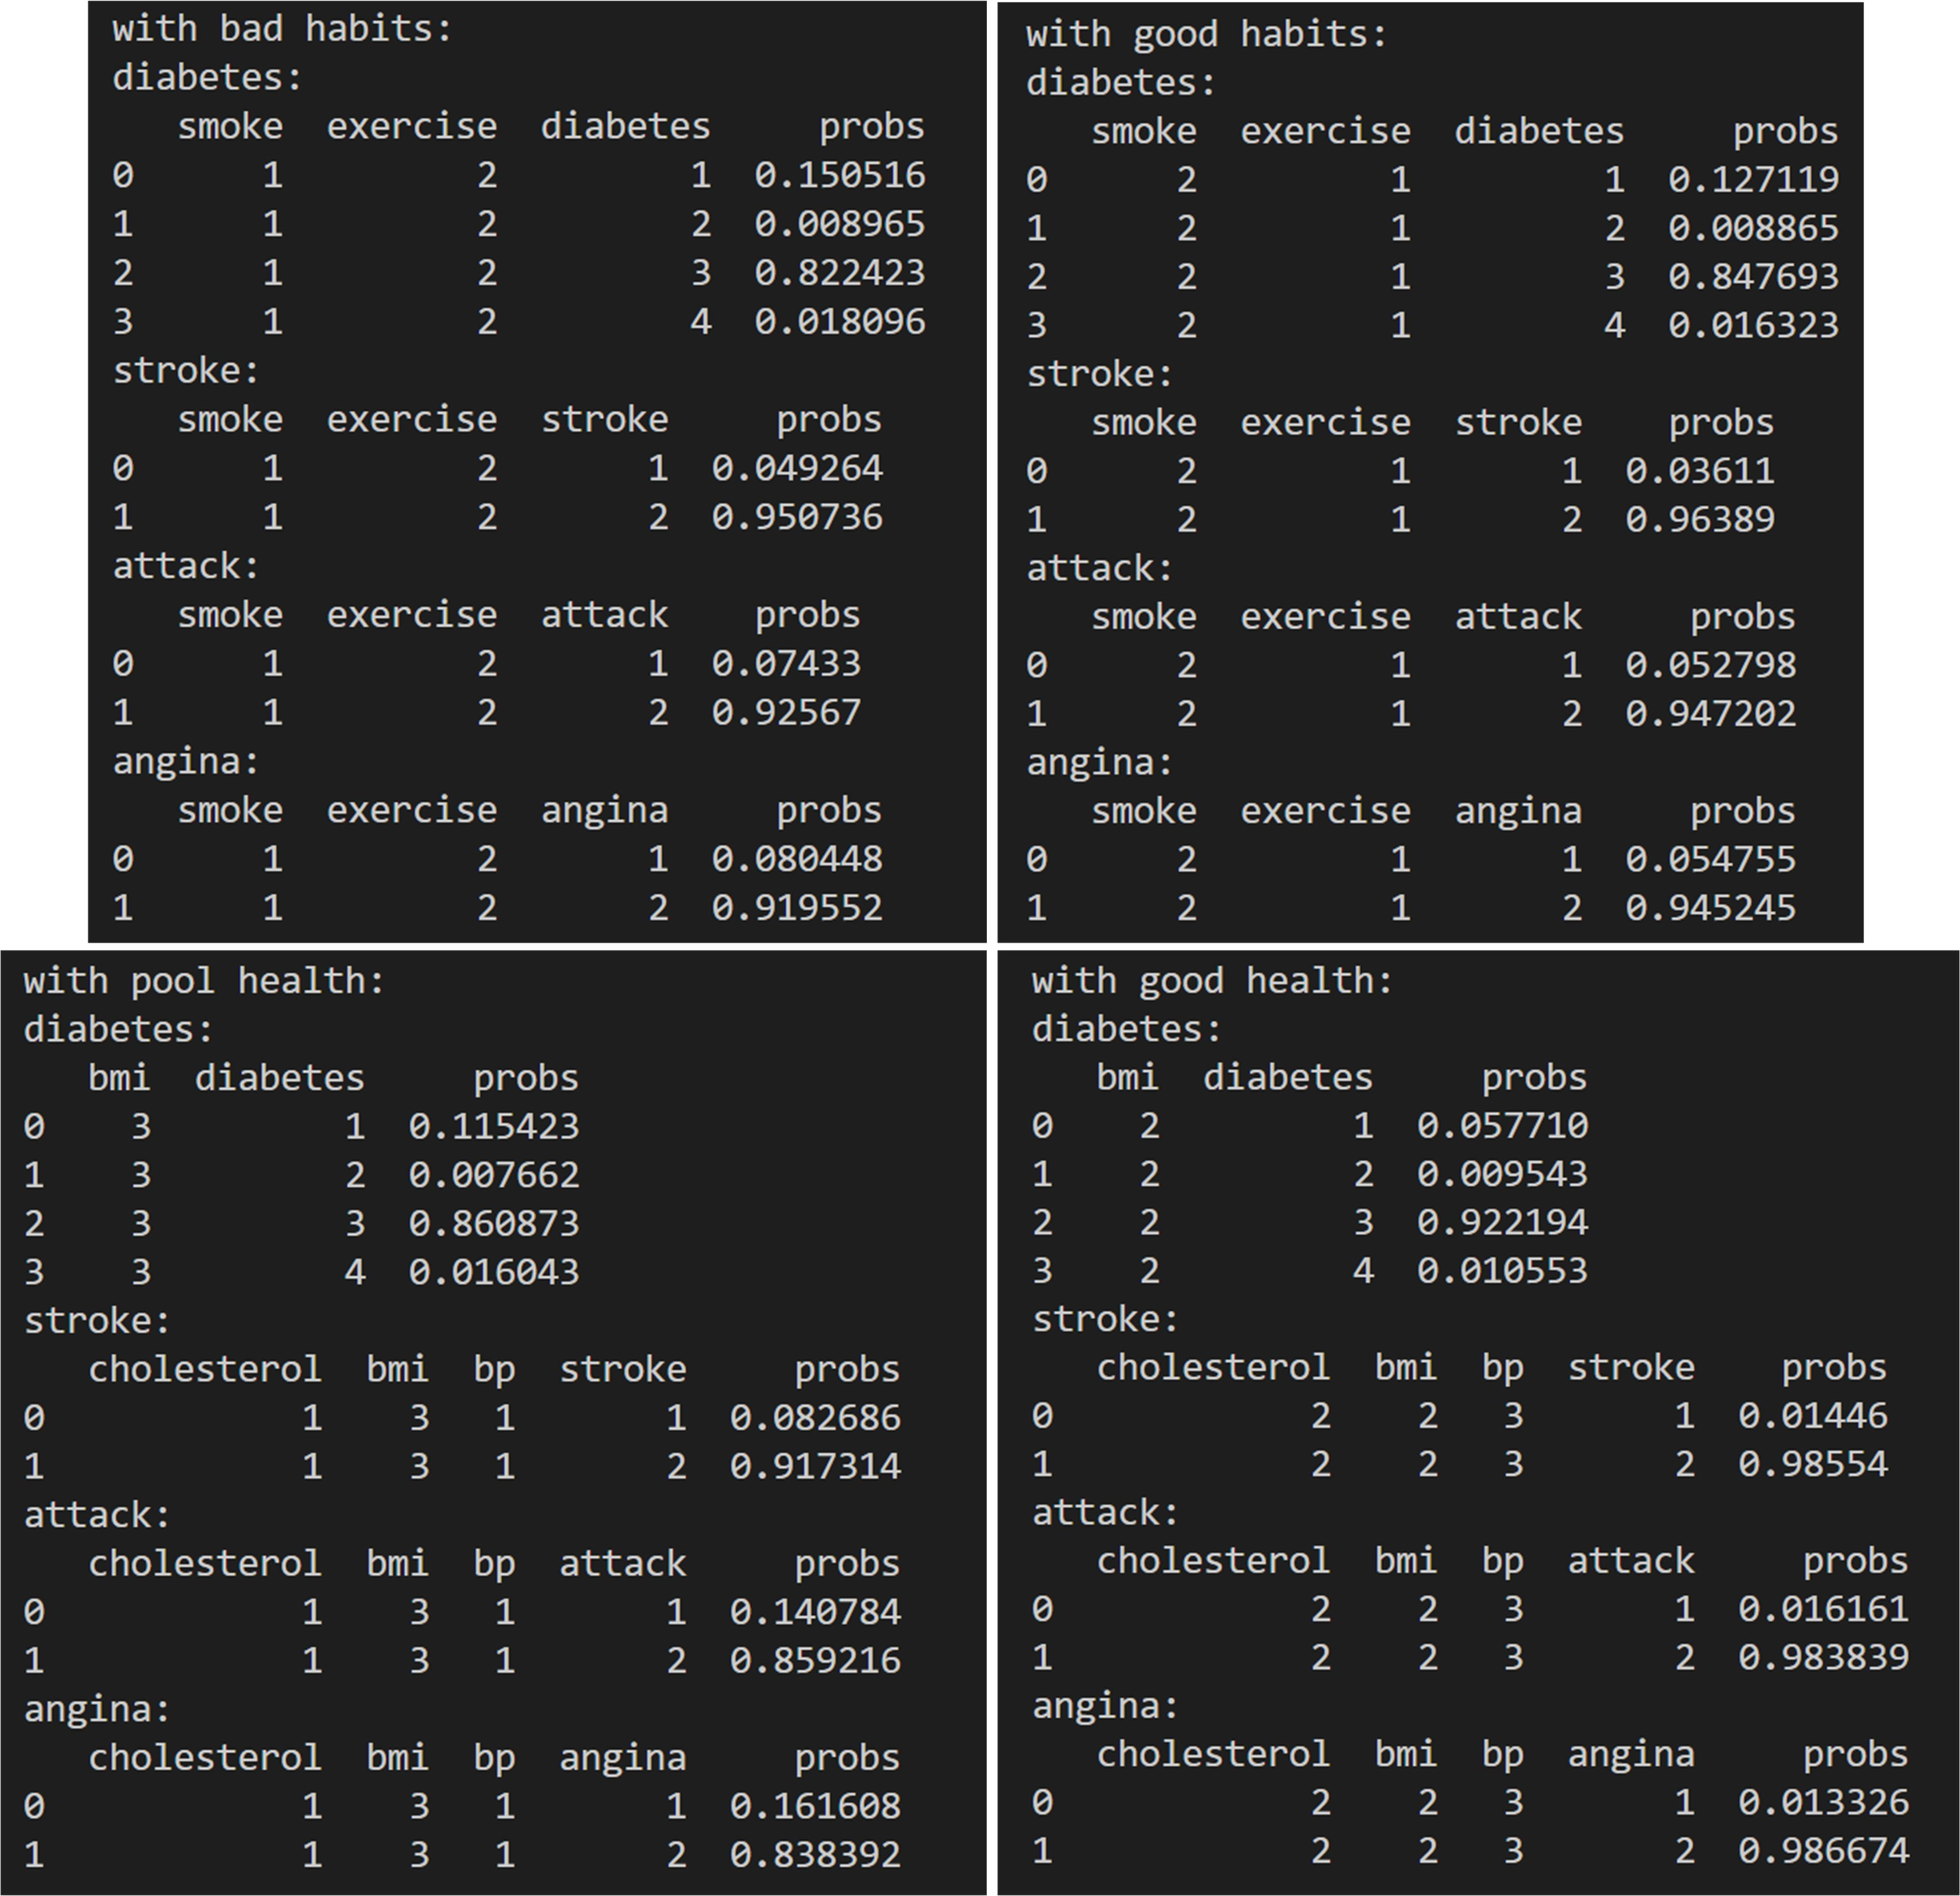
\includegraphics[width=0.95\linewidth]{T2.jpg}
        \caption{Results for Question 2.}
        \label{fig:Q2}
     \end{figure}
%------------------------------
~\\
\textbf{Q3 Answer:} 

The  effect that a person's income has on their probability of having one of the four health outcomes are evaluated and the comparations are shown in Figure~\ref{fig:Q3}. We can conclude that the higher a person's income status is ,the less probabilities to have diseases problem. But the people who earn 10000-15000\$ seem to be more likely to have diseases problem compared to the people who earn less than 10000\$.
\begin{figure}[H]
    \centering
    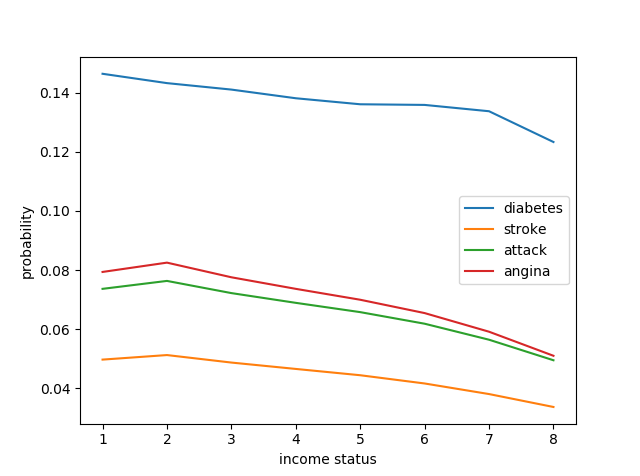
\includegraphics[width=0.65\linewidth]{Figure_T3.png}
    \caption{Results for Question 3.}
    \label{fig:Q3}
 \end{figure}

 %------------------------------

 ~\\
 \textbf{Q4 Answer:} 

As there are no links in the graph between the habits (smoking and exercise) and the outcomes, it can be infered that the effects of smoking and exercise on health problems are ignored, in other words, an assumption that smoking and exercise have no effects on health problems is made.  Test for the validity of these assumptions is made by adding edges from smoking to each of the four outcomes and edges from exercise to each of the four outcomes.

The probability of the outcome if I have bad habits or good habits and the probability of the outcome if I have poor health or good health are shown in Table~\ref{table:Q4}. The output of the code for question 2 are shown in Figure~\ref{fig:Q4}.

\begin{table}[H]
    \centering
    \begin{tabular}{|c|c|c|c|c|c|}
    \hline
    \multicolumn{2}{|c|}{health outcomes} & bad habits & good habits & pool health & good health \\ \hline
    \multirow{4}{*}{diabetes}       & 1   & 21.09\%    & 9.855\%     & 12.35\%     & 5.417\%     \\ \cline{2-6} 
                                    & 2   & 6.915\%    & 0.9884\%    & 0.7460\%    & 0.9731\%    \\ \cline{2-6} 
                                    & 3   & 76.07\%    & 87.76\%     & 85.24\%     & 92.60\%     \\ \cline{2-6} 
                                    & 4   & 2.145\%    & 1.399\%     & 1.664\%     & 1.014\%     \\ \hline
    \multirow{2}{*}{stroke}         & 1   & 7.804\%    & 2.421\%     & 8.426\%     & 1.400\%     \\ \cline{2-6} 
                                    & 2   & 92.20\%    & 97.57\%     & 91.57\%     & 98.60\%     \\ \hline
    \multirow{2}{*}{heart attack}   & 1   & 12.12\%    & 3.102\%     & 14.22\%     & 1.547\%     \\ \cline{2-6} 
                                    & 2   & 87.88\%    & 96.90\%     & 85.78\%     & 98.45\%     \\ \hline
    \multirow{2}{*}{angina}         & 1   & 11.90\%    & 3.68\%      & 16.30\%     & 1.294\%     \\ \cline{2-6} 
                                    & 2   & 88.10\%    & 96.32\%     & 83.70\%     & 98.71\%     \\ \hline
    \end{tabular}
    \caption{Results for Question 4.}
    \label{table:Q4}
\end{table}

    
\begin{figure}[H]
    \centering
    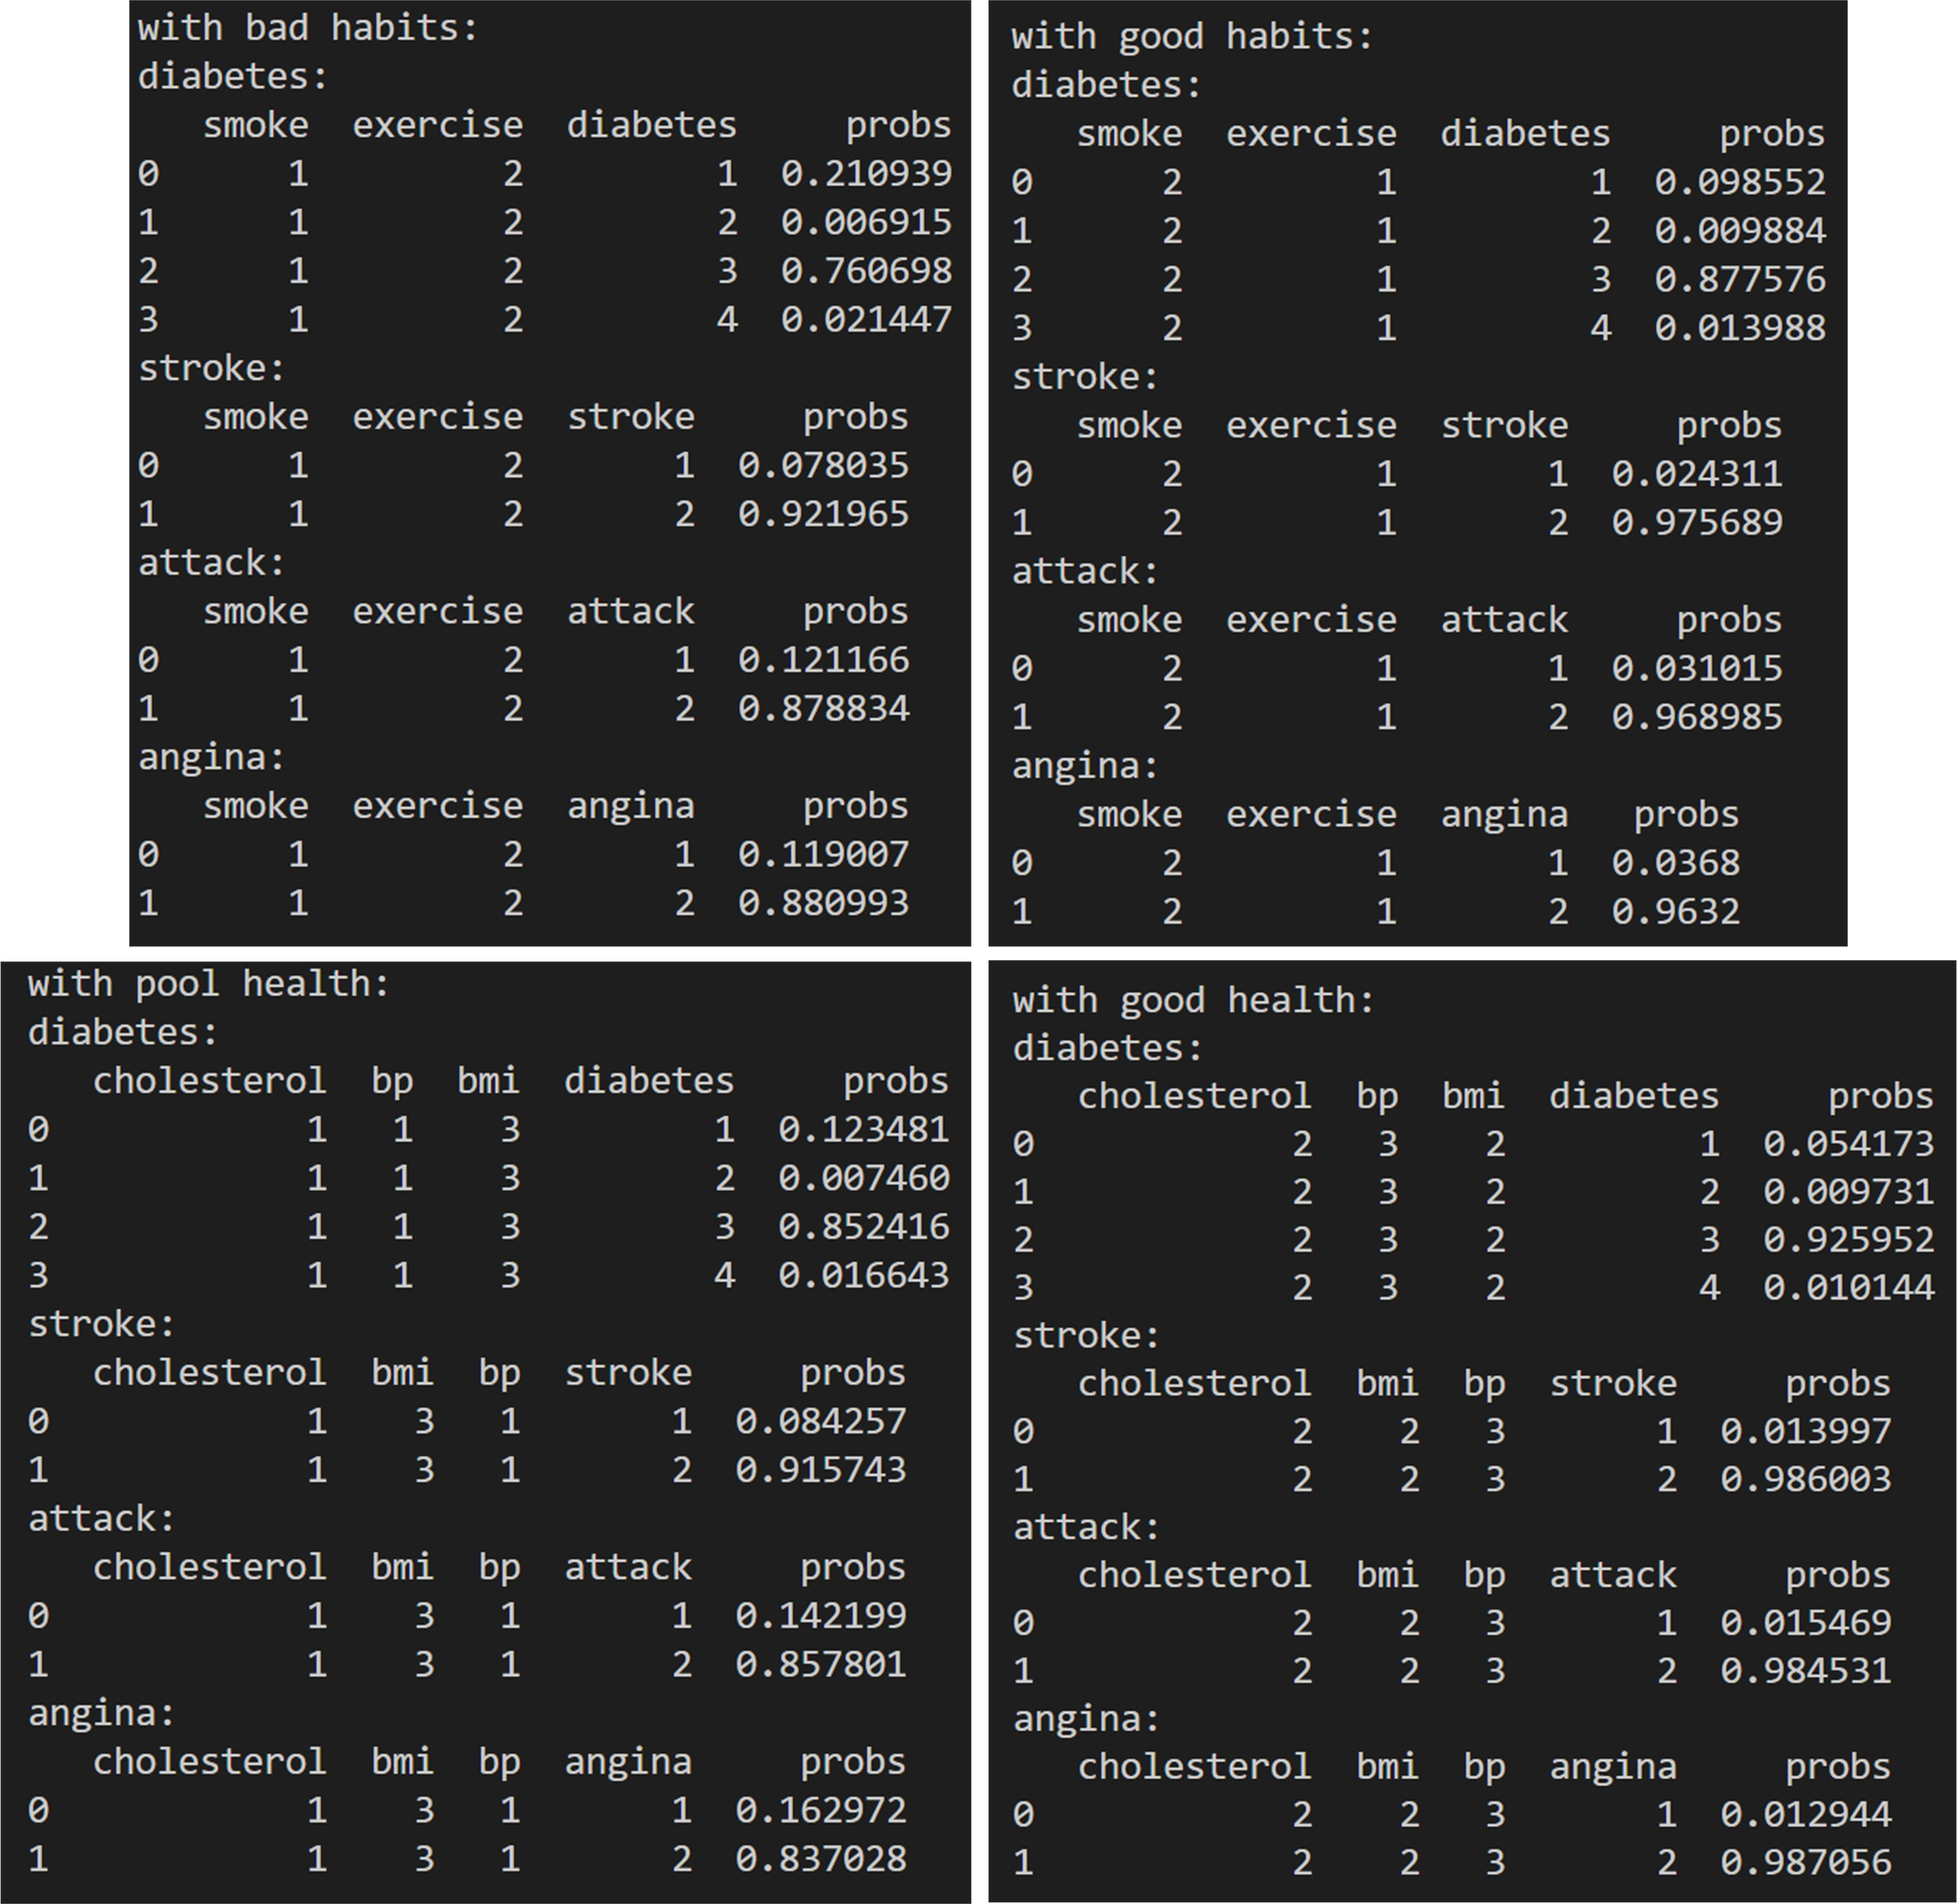
\includegraphics[width=0.95\linewidth]{T4.jpg}
    \caption{Results for Question 4.}
    \label{fig:Q4}
\end{figure}

Compare Table~\ref{table:Q4} and Table~\ref{table:Q2}, we can find that habits have significant impacts on the health outcome, while health status do not. For habits and outcomes, we can find that with good habits the morbidity will decrease and with bad habits it will increase, which means that there are some dependences between habits and outcomes and the assumption of habits is not valid. But for the health status and outcomes, the assumption that health status and outcomes are independent is valid.
%------------------------------

~\\
\textbf{Q5 Answer: }

As there are no edges between the four outcomes, it can be infered that the effects between four outcomes are ignored, in other words, an assumption that one outcome have no effects on others is made. 

The output of the code for question 5 are shown in Figure~\ref{fig:Q5}.

\begin{figure}[H]
    \centering
    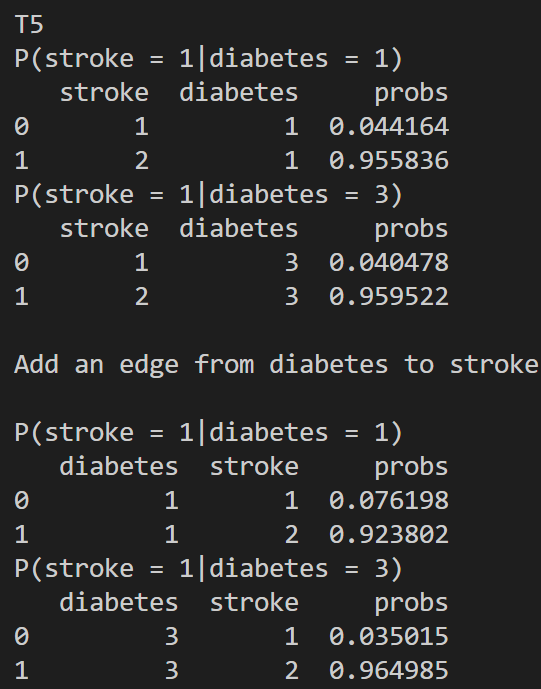
\includegraphics[width=0.35\linewidth]{T5.png}
    \caption{Results for Question 5.}
    \label{fig:Q5}
\end{figure}

From the results we can find that a person with diabetes problem is much more likely to face stroke problem, which means that the diabetes and stroke are correlative and the assumption that diabetes and stroke are independent is invalid.
%------------------------------

% \section{Discussion \& Conclusion}



\end{document} % DONE WITH DOCUMENT!


%%%%%%%%%%
PERSONAL FAVORITE LAB WRITE-UP STRUCTURE
%%%%%%%%%%
\section{Introduction}
	% No Text Here
	\subsection{Purpose}
		% Lab objective
	\subsection{Equipment}
		% Any and all equipment used (specific!)
	\subsection{Procedure}
		% Overview of the procedure taken (not-so-specific!)
\newpage
\section{Schematic Diagrams}
	% Any schematics, screenshots, block
   % diagrams used.  Possibly photos or
	% images could go here as well.
\newpage
\section{Experiment Data}
	% Depending on lab, program code would be
	% included here without the Estimated and
	% Actual Results.
	\subsection{Estimated Results}
		% Calculated. What it should be.
	\subsection{Actual Results}
		% Measured.  What it actually was.
\newpage
\section{Discussion \& Conclusion}
	% 3 Paragraphs:
		% Restate the objective of the lab
		% Discuss personal trials, errors, and difficulties
		% Conclude the lab


%%%%%%%%%%%%%%%%
COMMON COMMANDS:
%%%%%%%%%%%%%%%%
% IMAGES
begin{figure}[H]
   \begin{center}
      \includegraphics[width=0.6\textwidth]{RTL_SCHEM.png}
   \end{center}
\caption{A screenshot of the RTL Schematics produced from the Verilog code.}
\label{RTL}
\end{figure}

% SUBFIGURES IMAGES
\begin{figure}[H]
  \centering
  \subfloat[LED4 Period]{\label{fig:Per4}\includegraphics[width=0.4\textwidth]{period_led4.png}} \\
  \subfloat[LED5 Period]{\label{fig:Per5}\includegraphics[width=0.4\textwidth]{period_led5.png}}
  \subfloat[LED6 Period]{\label{fig:Per6}\includegraphics[width=0.4\textwidth]{period_led6.png}}
  \caption{Period of LED blink rate captured by osciliscope.}
  \label{fig:oscil}
\end{figure}

% INSERT SOURCE CODE
\lstset{language=Verilog, tabsize=3, backgroundcolor=\color{mygrey}, basicstyle=\small, commentstyle=\color{BrickRed}}
\lstinputlisting{MODULE.v}

% TEXT TABLE
\begin{table}
\begin{center}
\begin{tabular}{|l|c|c|l|}
	x & x & x & x \\ \hline
	x & x & x & x \\
	x & x & x & x \\ \hline
\end{tabular}
\caption{Caption}
\label{label}
\end{center}
\end{table}

% MATHMATICAL ENVIRONMENT
$ 8 = 2 \times 4 $

% CENTERED FORMULA
\[  \]

% NUMBERED EQUATION
\begin{equation}
	
\end{equation}

% ARRAY OF EQUATIONS (The splat supresses the numbering)
\begin{align*}
	
\end{align*}

% NUMBERED ARRAY OF EQUATIONS
\begin{align}
	
\end{align}

% ACCENTS
\dot{x} % dot
\ddot{x} % double dot
\bar{x} % bar
\tilde{x} % tilde
\vec{x} % vector
\hat{x} % hat
\acute{x} % acute
\grave{x} % grave
\breve{x} % breve
\check{x} % dot (cowboy hat)

% FONTS
\mathrm{text} % roman
\mathsf{text} % sans serif
\mathtt{text} % Typewriter
\mathbb{text} % Blackboard bold
\mathcal{text} % Caligraphy
\mathfrak{text} % Fraktur

\textbf{text} % bold
\textit{text} % italic
\textsl{text} % slanted
\textsc{text} % small caps
\texttt{text} % typewriter
\underline{text} % underline
\emph{text} % emphasized

\begin{tiny}text\end{tiny} % Tiny
\begin{scriptsize}text\end{scriptsize} % Script Size
\begin{footnotesize}text\end{footnotesize} % Footnote Size
\begin{small}text\end{small} % Small
\begin{normalsize}text\end{normalsize} % Normal Size
\begin{large}text\end{large} % Large
\begin{Large}text\end{Large} % Larger
\begin{LARGE}text\end{LARGE} % Very Large
\begin{huge}text\end{huge}   % Huge
\begin{Huge}text\end{Huge}   % Very Huge


% GENERATE TABLE OF CONTENTS AND/OR TABLE OF FIGURES
% These seem to have some issues with the "revtex4" document class.  To use, change
% the very first line of this document to "article" like this:
% \documentclass[aps,letterpaper,10pt]{article}
\tableofcontents
\listoffigures
\listoftables

% INCLUDE A HYPERLINK OR URL
\url{http://www.derekhildreth.com}
\href{http://www.derekhildreth.com}{Derek Hildreth's Website}

% FOR MORE, REFER TO THE "LINUX CHEAT SHEET.PDF" FILE INCLUDED!
